% report.tex
% main file for the project report.

\documentclass[a4paper,titlepage,12pt]{scrreprt}

% utf-8
\usepackage{polyglossia}
\setdefaultlanguage[babelshorthands]{ngerman}
\usepackage{fontspec}
\usepackage{pdfpages}

%Needed to wrap text around images, used for personas
\usepackage{wrapfig}

%Used to avoid page breaks with each chapter
\usepackage{etoolbox}
\makeatletter
\patchcmd{\chapter}{\if@openright\cleardoublepage\else\clearpage\fi}{}{}{}
\makeatother

% german names
\usepackage{ngerman}

% colored links
\usepackage{color}
\usepackage[colorlinks]{hyperref}
\definecolor{grey}{rgb}{0.2,0.2,0.2}
\definecolor{orange}{rgb}{1,0.3,0}
\definecolor{turqoise}{rgb}{0,0.7,0.5}

% code listings
\usepackage{listings}
\lstset{%
	basicstyle={\ttfamily \small},
	breaklines=true,
	commentstyle=\color{grey},
	keywordstyle=\color{orange},
	language=C,
	numbers=left,
	showspaces=false,
	stringstyle=\color{turqoise},
	xleftmargin=20pt
}

% graphics
\usepackage{graphicx}
\graphicspath{{images/}}

% fancy headers and footers
\usepackage{fancyhdr}
\pagestyle{fancy}
% clear style
\fancyhead{}
\fancyfoot{}
% new style
\renewcommand{\chaptermark}[1]{%
	\markboth{\thechapter.\ #1}{}
}
\renewcommand{\sectionmark}[1]{%
	\markright{\thesection.\ #1}{}
}
\renewcommand{\headrulewidth}{0.5pt}
\renewcommand{\footrulewidth}{0.5pt}
\fancyhead[LE,RO]{\rightmark}
\fancyhead[LO,RE]{\leftmark}
\fancyfoot[LE,RO]{\thepage}
\fancyfoot[LO,RE]{SWE Labor - Tobias Kerst, Gregor Rydzynski}
\fancypagestyle{plain}{%
	\fancyhf{}
	\renewcommand{\headrulewidth}{0pt}
	\renewcommand{\footrulewidth}{0.5pt}
	\fancyfoot[LE,RO]{\thepage}
	\fancyfoot[LO,RE]{SWE Sommersemester 2016}
}

% no indented paragraphs
\usepackage{parskip}

% TODO: what's this?
\setkomafont{disposition}{\normalfont\bfseries}

% for verbatiminput
\usepackage{verbatim}

% not yet used
%\input{src/cmd}

\begin{document}

\titlehead{
	
\includegraphics[width=0.9\linewidth]{hska_logo}
}

\title{Software-Engineering Labor}
\subtitle{Entwicklung des Lern-Quiz-Computer Spiels}
\author{%
	Tobias Kerst (47646)\\
	Gregor Rydzynski (44354)\\
	Gruppe 20
}
\date{Sommersemester 2016}
\publishers{
    \textbf{Dozent:} Prof. Dr. Th. Fuchß
}
\maketitle

\clearpage

\begingroup
\hypersetup{linkcolor=black}
\tableofcontents
\endgroup

\clearpage

\chapter{Analyse}\label{chap:Analyse}

\section{Use Case Beschreibungen}
\begin{figure}[h]
  \begin{center}
    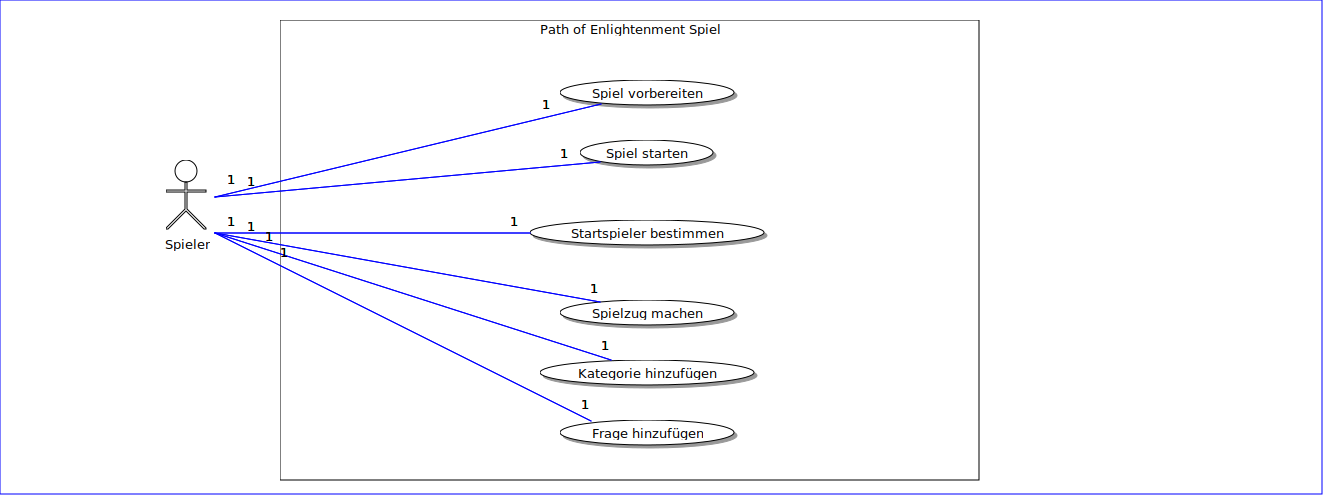
\includegraphics[width=0.9\textwidth]{UseCaseDiagram}
    \caption{Use Case Diagram für das Spiel}
  \end{center}
\end{figure}

\subsection{Use Case: Spiel vorbereiten}
\begin{labeling}[:]{Vorbedingungen}
\item [Akteure] Spieler
\item [Priorität] Wichtig
\item [Beschreibung] Die Spieler wählen aus den vorhandenen Kategorien 4 aus. Die Fragen jeder Kategorie werden gemischt. Jeder Spieler wählt eine Farbe für sich aus.
\item [Vorbedingungen] Es existieren mindestens 4 Kategorien
\item [Offene Punkte] Was wird gemacht, wenn weniger als 4 Kategorien existieren.
\end{labeling}

\subsection{Use Case: Startspieler bestimmen}
\begin{labeling}[:]{Vorbedingungen}
\item [Akteure] Spieler
\item [Priorität] Essentiell
\item [Beschreibung] Die Spieler würfeln der Reihe nach einmal mit einem Würfel. Der Spieler, dessen Wurf die höchste Augenzahl aufweist, darf beginnen. Sollten mehrere Spieler die gleiche höchste Augenzahl gewürfelt haben, so müssen nur diese erneut untereinander auswürfeln, wer beginnt. Dies wird so lange gemacht, bis ein Spieler eindeutig als Startspieler ausgemacht ist.
\item [Vorbedingungen] Spiel gestartet
\item [Offene Punkte]
\end{labeling}

\subsection{Use Case: Spielzug machen}
\begin{labeling}[:]{Vorbedingungen}
\item [Akteure] Spieler
\item [Priorität] Essentiell
\item [Beschreibung] Hat ein Spieler alle 3 Wissensstreiter auf seinen Heimatfeldern, darf er in diesem Zug 3 Mal würfeln um einen Wissensstreiter ins Spiel zu bringen. Er bringt einen seiner Wissensstreiter ins Spiel, indem er eine 6 würfelt. Würfelt er innerhalb dieser 3 Würfe eine 6, so wird einer seiner Wissensstreiter auf dem Pfad des Wissens platziert (auf dem entsprechenden Feld mit der Spielerfarbe) und sein Zug ist beendet. Sollte der Spieler nach den 3 Würfen keine 6 gewürfelt haben, so wird der Zug beendet und der nächste Spieler nach dem Uhrzeigersinn ist an der Reihe. \\
Hat ein Spieler mindestens einen seiner Wissensstreiter auf dem Pfad des Wissens, so würfelt er nur ein Mal. Würfelt er eine 6 und hat noch einen Wissensstreiter auf einem Heimatfeld, so muss er diesen ins Spiel bringen.
\\
Andernfalls kann der Spieler einen seiner Wissensstreiter um die gewürfelte Augenzahl auf dem Pfad nach vorne setzen. Er darf jedoch keinen seiner Wissensstreiter auf ein Feld setzen, auf dem sich schon ein anderer Wissensstreiter von ihm befindet.
\\
Kommt einer der Wissensstreiter auf ein Feld, auf dem bereits ein Wissensstreiter eines anderes Spieler steht, so beginnt eine \textbf{Fragerunde} mit diesem Mitspieler. Dies gilt auch dann, wenn ein Spieler einen seiner Wissensstreiter gerade erst von seinen Heimatfeldern auf den Pfad bringt und sein Startfeld auf dem Pfad durch einen anderen Spieler belegt ist.
\item [Vorbedingungen] Vorheriger Spielzug ist beendet worden. Bei erstem Spielzug: Startspieler bestimmt.
\item [Offene Punkte]
\end{labeling}

\subsection{Use Case: Fragerunde}
\begin{labeling}[:]{Vorbedingungen}
\item [Akteure] Spieler, Gegenspieler
\item [Priorität] Essentiell
\item [Beschreibung] Der Spieler stellt seinem Mitspieler (auch Geprüfter genannt) eine Frage aus einer der 4 Kategorien. Kann der Geprüfte die Frage beantworten, so kann dieser seinen Wissensstandanzeiger für die gewählte Kategorie auf die nächst höhere Stufe setzen. Ist die höchste Stufe bereits erreicht worden, so kann ein Wissensstandanzeiger in einer anderen Kategorie (die von dem Geprüften bestimmt wird) erhöht werden. Im Anschluss wird der Wissensstreiter des Geprüften auf dessen Startfeld gesetzt. Befindet sich dort bereits ein Wissensstreiter des selben Spielers, so wandert der Wissensstreiter auf eines der Heimatfelder.
\\
Sollte der Geprüfte die Frage jedoch nicht korrekt beantworten können, wird der Wissensstandanzeiger eine Stufe herabgesetzt und der Wissensstreiter landet direkt auf einem der Heimatfelder. Im Anschluss muss der Fragestellende die selbe Frage beantworten. Wenn er sie richtig beantwortet, bleibt seine Spielfigur auf dem Feld stehen und ansonsten gelten die selben Regeln, wie bei dem Geprüften. \\

Hat nach dem Zug ein Spieler alle Wissensstandanzeiger auf der höchsten Stufe, so gewinnt dieser das Spiel und das Spiel ist beendet.
\item [Vorbedingungen]
\item [Offene Punkte]
\end{labeling}

\newpage{}
\subsection{Use Case: Kategorie hinzufügen}
\begin{labeling}[:]{Vorbedingungen}
\item [Akteure] Spieler
\item [Priorität] Unwichtig
\item [Beschreibung] Der Spieler kann eine eigene Kategorie hinzufügen, der dann Fragen zugeordnet werden können.
\item [Vorbedingungen]
\item [Offene Punkte]
\end{labeling}

\subsection{Use Case: Frage hinzufügen}
\begin{labeling}[:]{Vorbedingungen}
\item [Akteure] Spieler
\item [Priorität] Unwichtig
\item [Beschreibung] Der Spieler kann eine Frage erstellen und mit einer Antwort versehen. Dann wird diese Frage einer Kategorie zugeordnet.
\item [Vorbedingungen] Kategorie vorhanden
\item [Offene Punkte]
\end{labeling}

\section{Begründung für die Priorisierung}\label{sec:begruendung-prio}
Die letzten beiden Punkte wurden als \texttt{unwichtig} eingestuft, da diese das Spielerlebnis zwar verbessern und personalisieren würden, jedoch ein Spiel ohne diese Funktionalität voll spielbar ist.\\
Das Spiel kommt nicht ohne die als \texttt{essentiell} gekennzeichneten Use Cases aus, da es ohne diese unspielbar ist. Ohne den Use Case \emph{Fragerunde} zum Beispiel, würde das Spiel keinen Gewinner und damit auch kein Ende finden.\\
Die Spielvorbereitung ist wichtig, da hierüber das Spielgeschehen maßgeblich gesteuert wird, also wie viele Spieler, mit welchen Kategorien spielen, aber sind nicht essentiell, da man hier auch mit festen Werten ein spielbares Spiel entwickeln könnte, was jedoch wenig Freude bereiten würde.

\newpage
\section{Erste Iteration}
Für die erste Iteration werden lediglich die als \texttt{essentiell} priorisierten Use Cases implementiert. Dies sind die Folgenden

\begin{enumerate}
\item Startspieler bestimmen
\item Spielzug machen
\item Fragerunde
\end{enumerate}

Die Begründung für die Auswahl liegt in der Gewichtung, siehe hierzu \ref{sec:begruendung-prio}

\newpage
\section{Activity-Diagramme}
\subsection{Startspieler bestimmen}
\begin{figure}[h]
  \begin{center}
    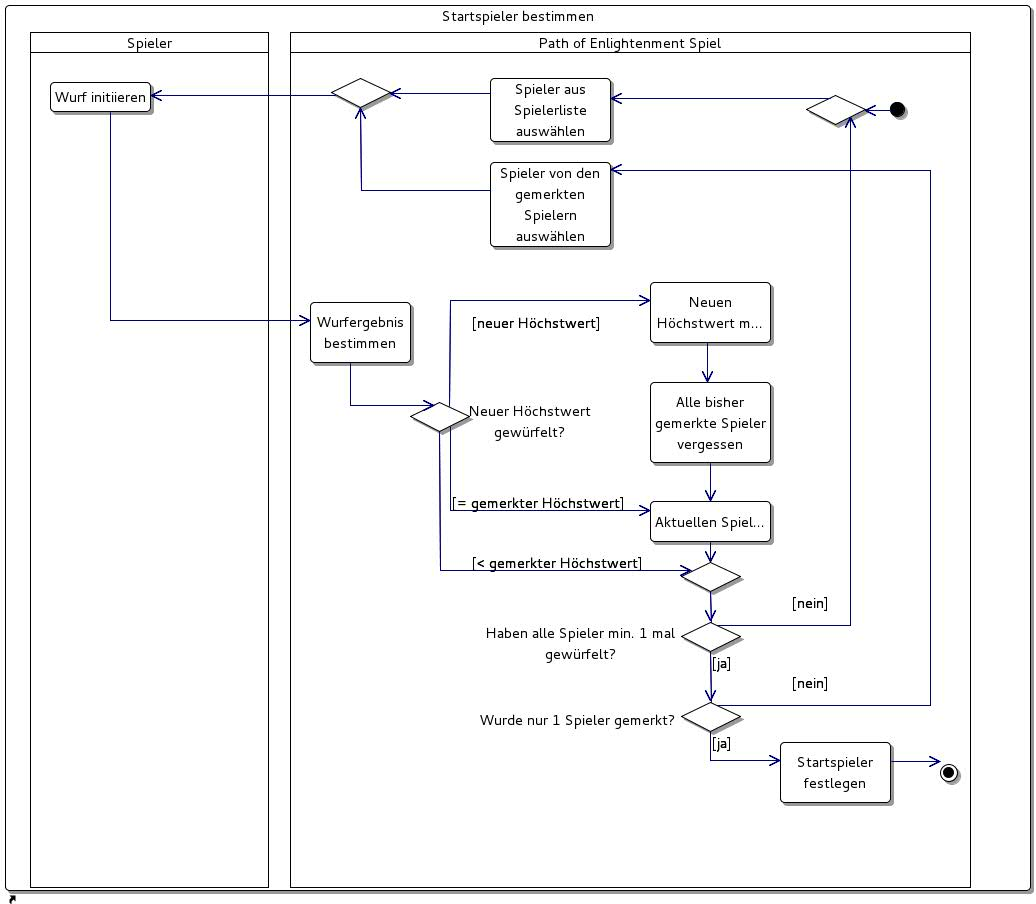
\includegraphics[width=0.9\textwidth]{diagrams/Startspieler_bestimmen}
  \end{center}
\end{figure}

\newpage
\subsection{Spielzug machen}
\begin{figure}[h]
  \begin{center}
    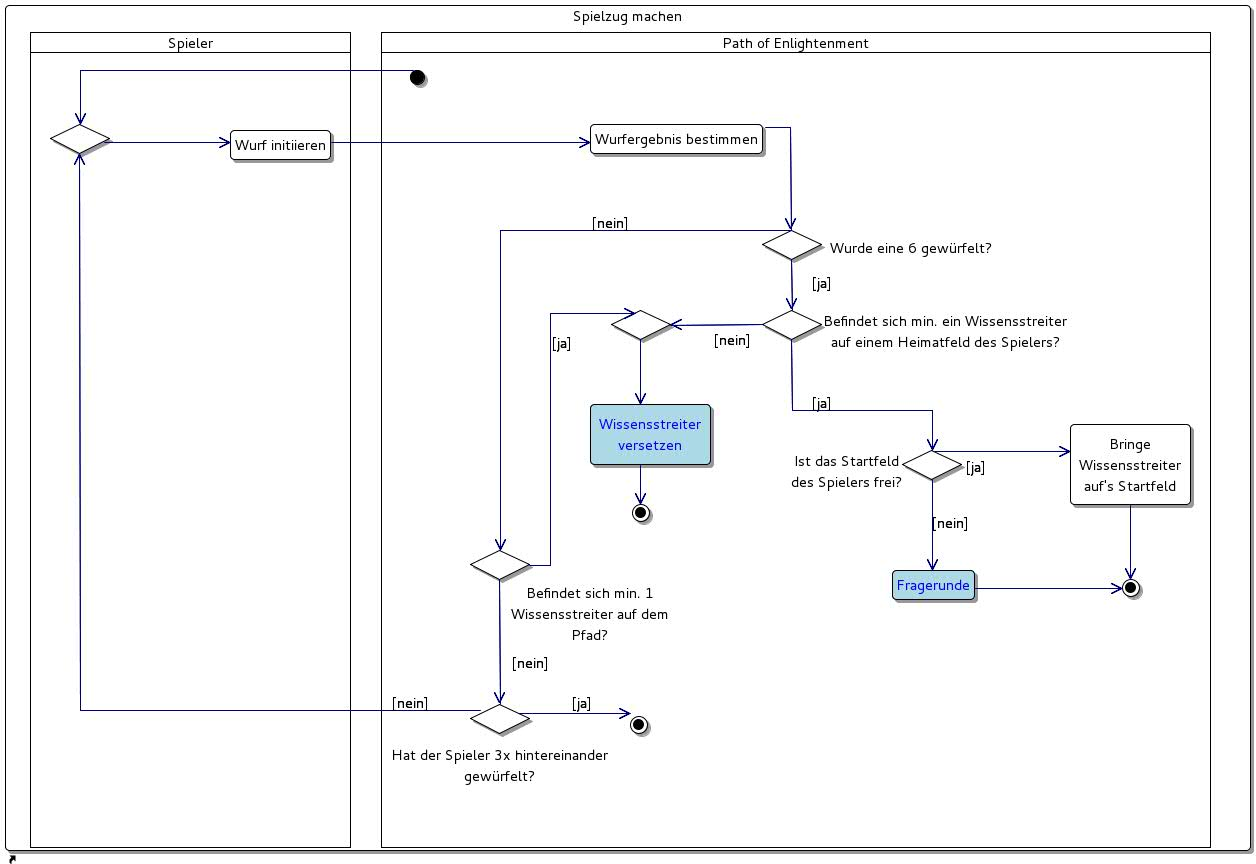
\includegraphics[width=0.9\textwidth]{diagrams/Spielzug_machen}
  \end{center}
\end{figure}

\newpage
\subsection{Fragerunde}
\begin{figure}[h]
  \begin{center}
    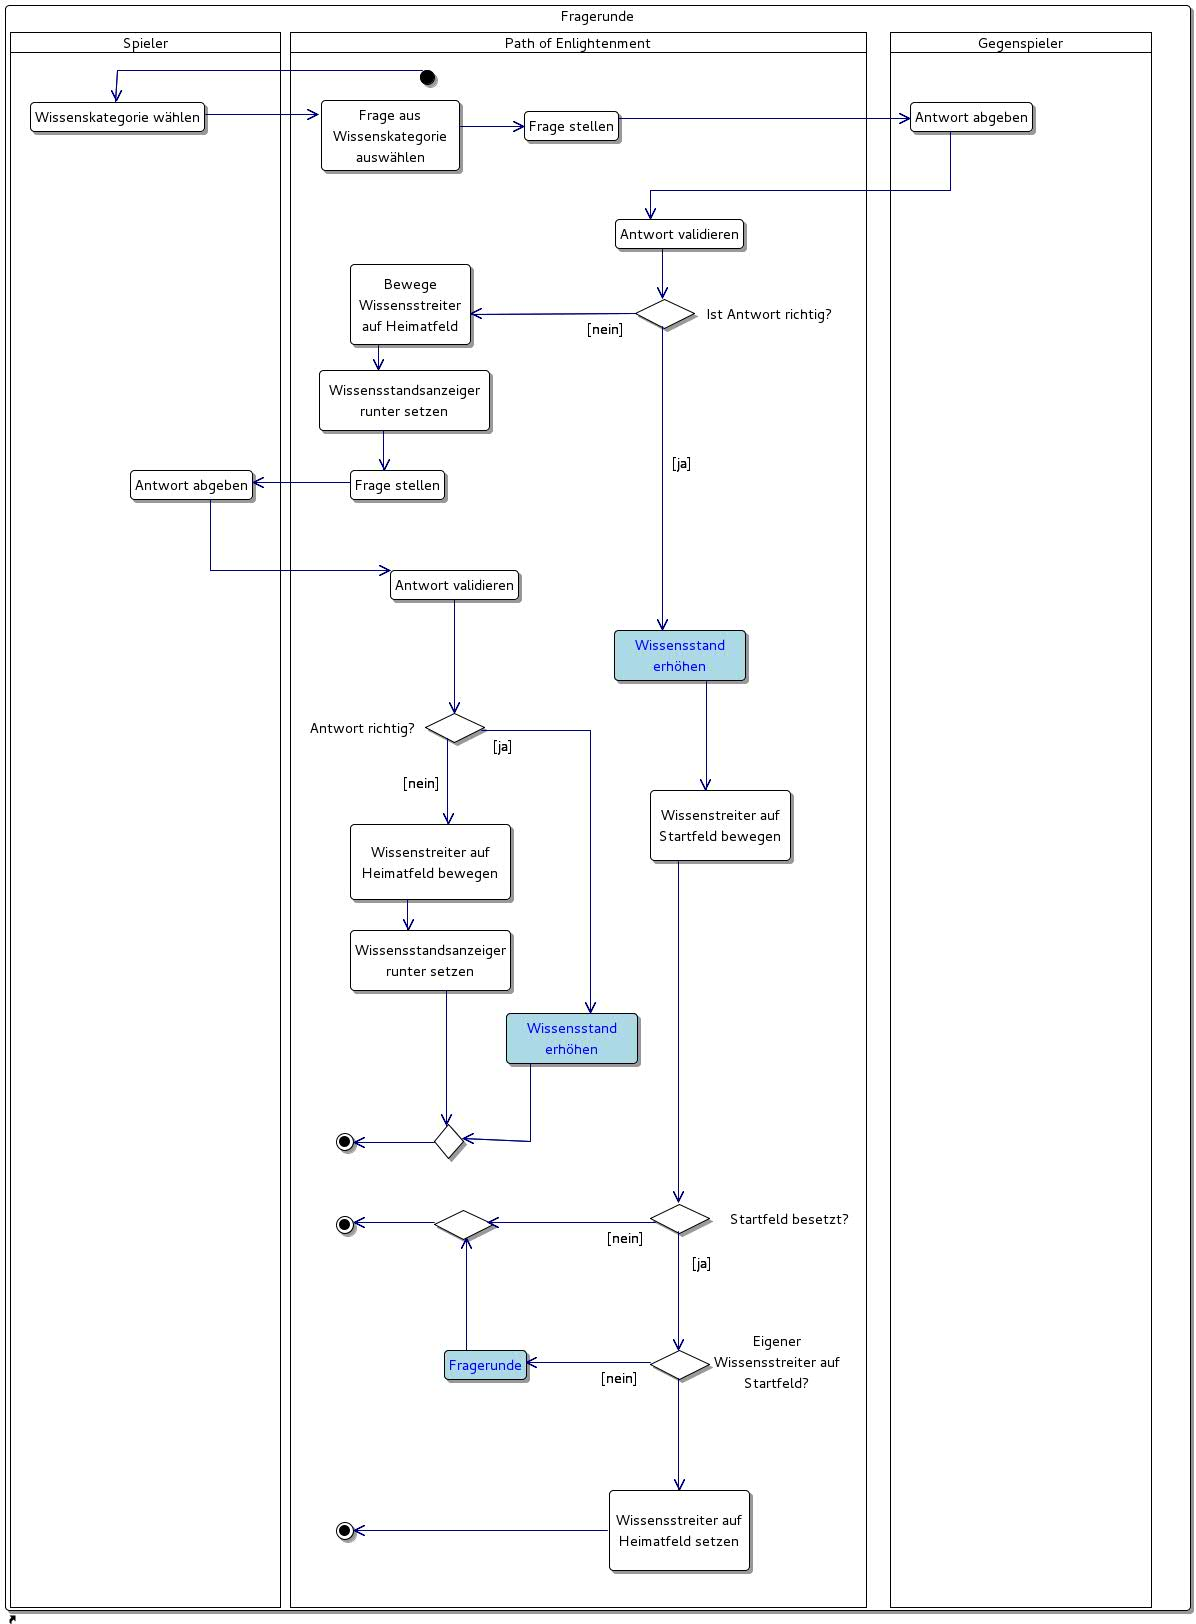
\includegraphics[width=0.8\textwidth]{diagrams/Fragerunde}
  \end{center}
\end{figure}

\newpage
\subsection{Wissensstreiter versetzen}
\begin{figure}[h]
  \begin{center}
    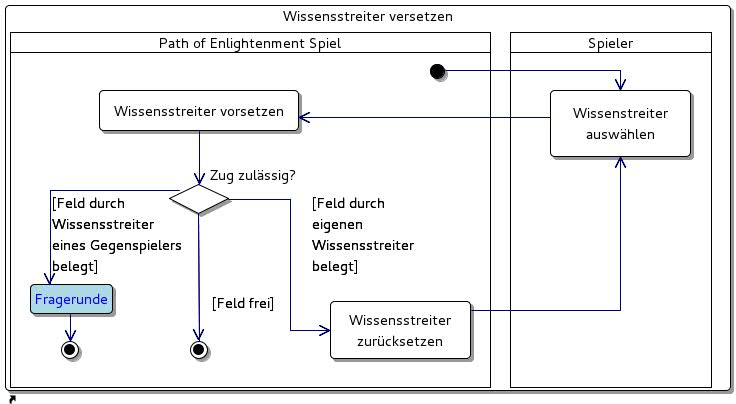
\includegraphics[width=0.9\textwidth]{diagrams/Wissensstreiter_versetzen}
  \end{center}
\end{figure}

\newpage
\subsection{Wissensstand erhöhen}
\begin{figure}[h]
  \begin{center}
    \includegraphics[width=0.9\textwidth]{diagrams/Wissensstand_erhöhen}
  \end{center}
\end{figure}

\newpage
\section{Objektmodell}
\begin{figure}[h]
  \begin{center}
    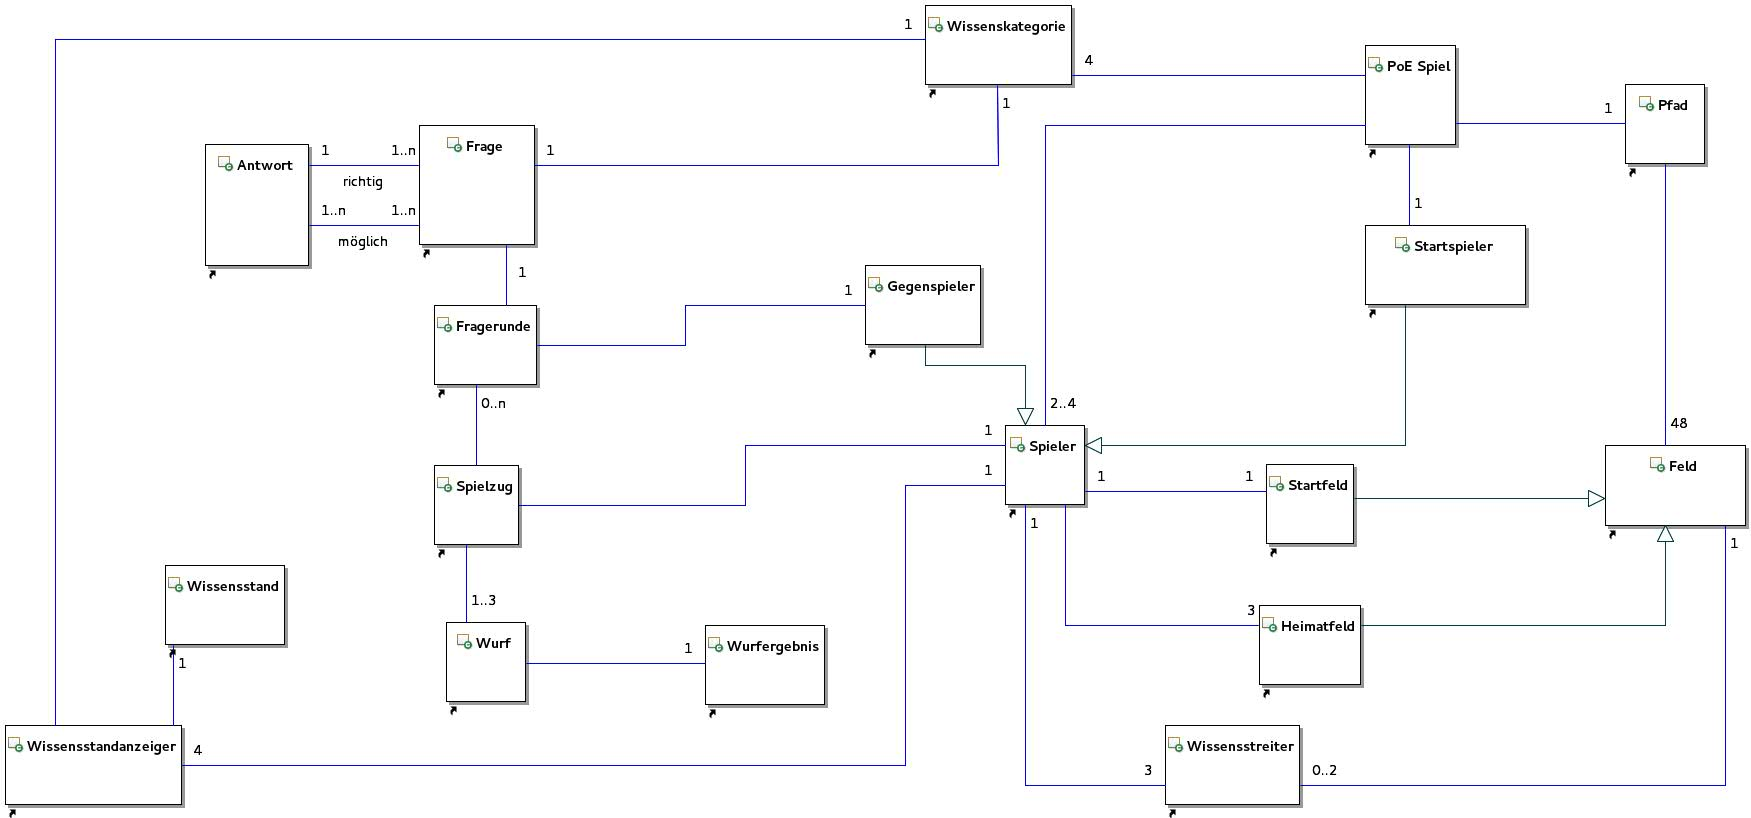
\includegraphics[width=0.9\textwidth]{diagrams/Objektmodell}
  \end{center}
\end{figure}

\newpage
\section{System-Sequenz-Diagramme}
\subsection{Startspieler bestimmen}
\begin{figure}[h]
  \begin{center}
    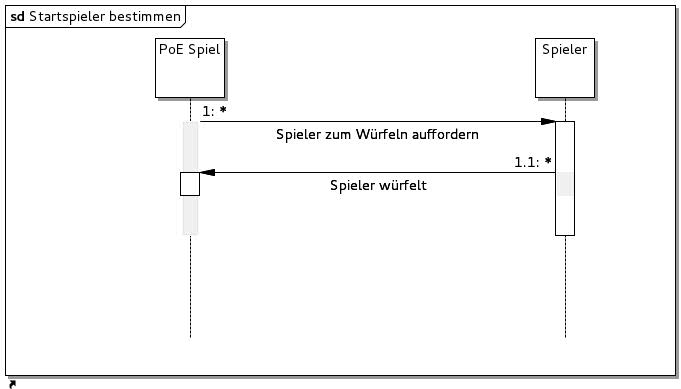
\includegraphics[width=0.9\textwidth]{diagrams/Startspieler_bestimmen_sequenz}
  \end{center}
\end{figure}

\subsubsection{Operation: Spieler zum Würfeln auffordern}
\begin{labeling}[:]{Verantwortlichkeit}
\item [Verantwortlichkeit] Ermöglicht einem Spieler zu würfeln.
\item [Referenzen] Use Case \texttt{Startspieler bestimmen}
\item [Output] 
\item [Vorbedingungen] keine
\item [Nachbedingungen] Der Spieler hat die Möglichkeit einen Wurf zu tätigen
\end{labeling}

\subsubsection{Operation: Spieler würfelt (Würfeln)}
\begin{labeling}[:]{Verantwortlichkeit}
\item [Verantwortlichkeit] Initiiert einen Wurf und bestimmt ein Wurfergebnis
\item [Referenzen] Use Cases \texttt{Startspieler bestimmen} und \texttt{Spielzug machen}
\item [Output] Wurfergebnis
\item [Vorbedingungen] Der Spieler ist an der reihe und darf würfeln
\item [Nachbedingungen] Es gibt ein Wurfergebnis für den aktuellen Wurf
\end{labeling}

\newpage
\subsection{Spielzug machen}
\begin{figure}[h]
  \begin{center}
    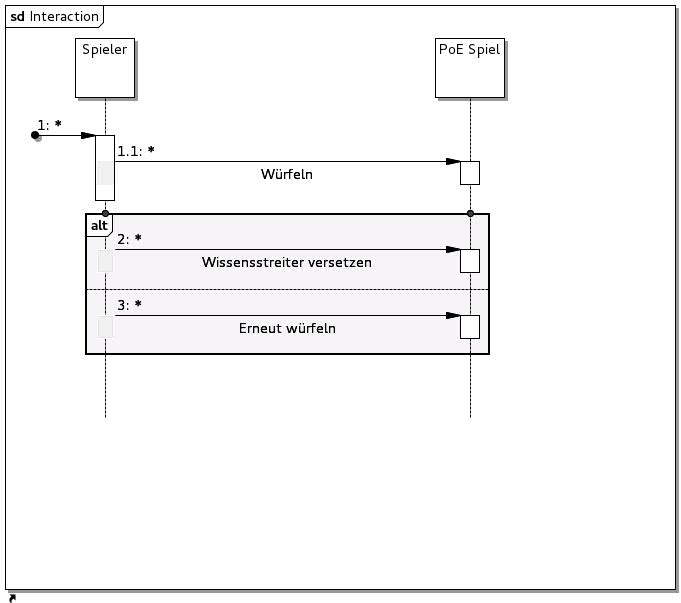
\includegraphics[width=0.9\textwidth]{diagrams/Spielzug_machen_sequenz}
  \end{center}
\end{figure}

\subsubsection{Operation: Erneut würfeln}
\begin{labeling}[:]{Verantwortlichkeit}
\item [Verantwortlichkeit] Initiiert einen neuen Wurf und bestimmt ein Wurfergebnis
\item [Referenzen] Use Case \texttt{Spielzug machen}
\item [Output] Wurfergebnis
\item [Vorbedingungen] Der Spieler hat noch keinen Wissensstreiter auf dem Pfad und noch keine 3 mal gewürfelt
\item [Nachbedingungen] Es gibt ein neues Wurfergebnis für den aktuellen Wurf, nach 3x würfeln ist der nächste Spieler dran oder ein Wissensstreiter wird versetzt
\end{labeling}

\subsubsection{Operation: Wissensstreiter versetzen}
\begin{labeling}[:]{Verantwortlichkeit}
\item [Verantwortlichkeit] Versetzt einen Wissensstreiter auf dem Pfad versetzt
\item [Referenzen] Use Case \texttt{Spielzug machen}
\item [Output] 
\item [Vorbedingungen] Der Spieler hat min. einen Wissensstreiter auf dem Pfad, mit dem ein Zug möglich ist
\item [Nachbedingungen] Der Wissensstreiter wurde versetzt und es wird ein neuer Spielzug oder eine Fragerunde initiiert
\end{labeling}

\newpage
\subsection{Fragerunde}
\begin{figure}[h]
  \begin{center}
    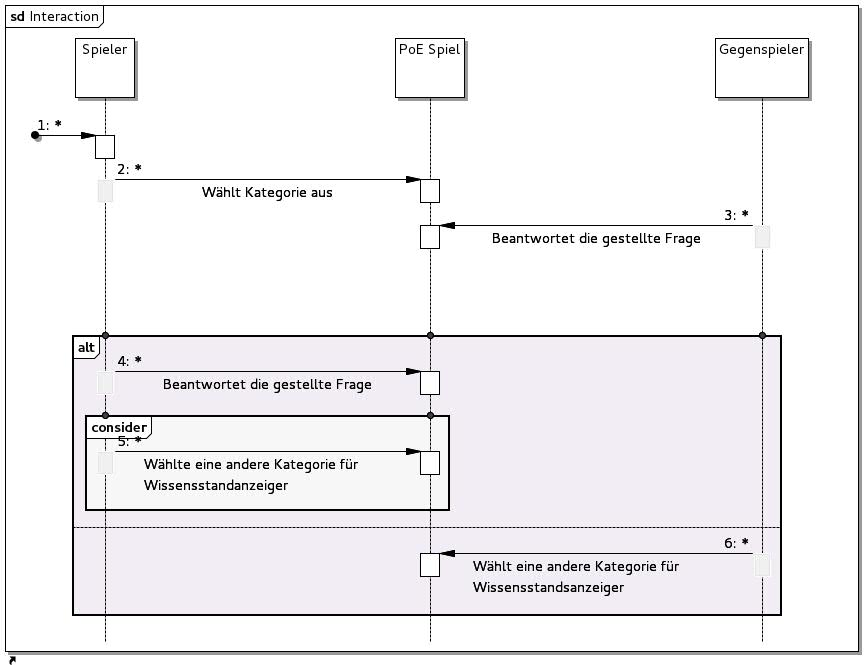
\includegraphics[width=0.8\textwidth]{diagrams/Fragerunde_sequenz}
  \end{center}
\end{figure}

\subsubsection{Operation: Wählt Kategorie aus}
\begin{labeling}[:]{Verantwortlichkeit}
\item [Verantwortlichkeit] Initiiert einen neuen Wurf und bestimmt ein Wurfergebnis
\item [Referenzen] Use Case \texttt{Fragerunde}
\item [Output] Gewählte Kategorie
\item [Vorbedingungen] Der Spieler ist auf ein Feld mit einem gegnerischen Wissensstreiter gekommen
\item [Nachbedingungen] Es wurde eine der 4 Wissenskategorien ausgewählt
\end{labeling}

\subsubsection{Operation: Beantwortet die gestellte Frage}
\begin{labeling}[:]{Verantwortlichkeit}
\item [Verantwortlichkeit] Es wird eine Antwort zu der Frage abgegeben
\item [Referenzen] Use Case \texttt{Fragerunde}
\item [Output] Antwort auf die Frage
\item [Vorbedingungen] Es wurde eine Frage gestellt
\item [Nachbedingungen] Die Antwort wird auf Richtigkeit geprüft. Wenn die Frage richtig beantwortet wurde, darf der Wissensstandanzeiger für die Kategorie erhöht werden. Falls die Kategorie schon auf dem Maximum ist darf der Spieler eine andere Kategorie auswählen.
\end{labeling}

\subsubsection{Operation: Wählt eine andere Kategorie für Wissensstandanzeiger}
\begin{labeling}[:]{Verantwortlichkeit}
\item [Verantwortlichkeit] Es wird eine andere Kategorie für die der Wissensstandanzeiger erhöht werden soll ausgewählt
\item [Referenzen] Use Case \texttt{Fragerunde}
\item [Output] Neu gewählte Kategorie
\item [Vorbedingungen] Der Wissensstand für die aktuelle Kategorie ist auf max.
\item [Nachbedingungen] Eine andere Wissenskategorie, für die der Wissensstandanzeiger nicht die max. Stufe hat, wurde ausgewählt
\end{labeling}
\chapter{Design}\label{chap:Design}

\section{Architektur}
\begin{figure}[h]
  \begin{center}
    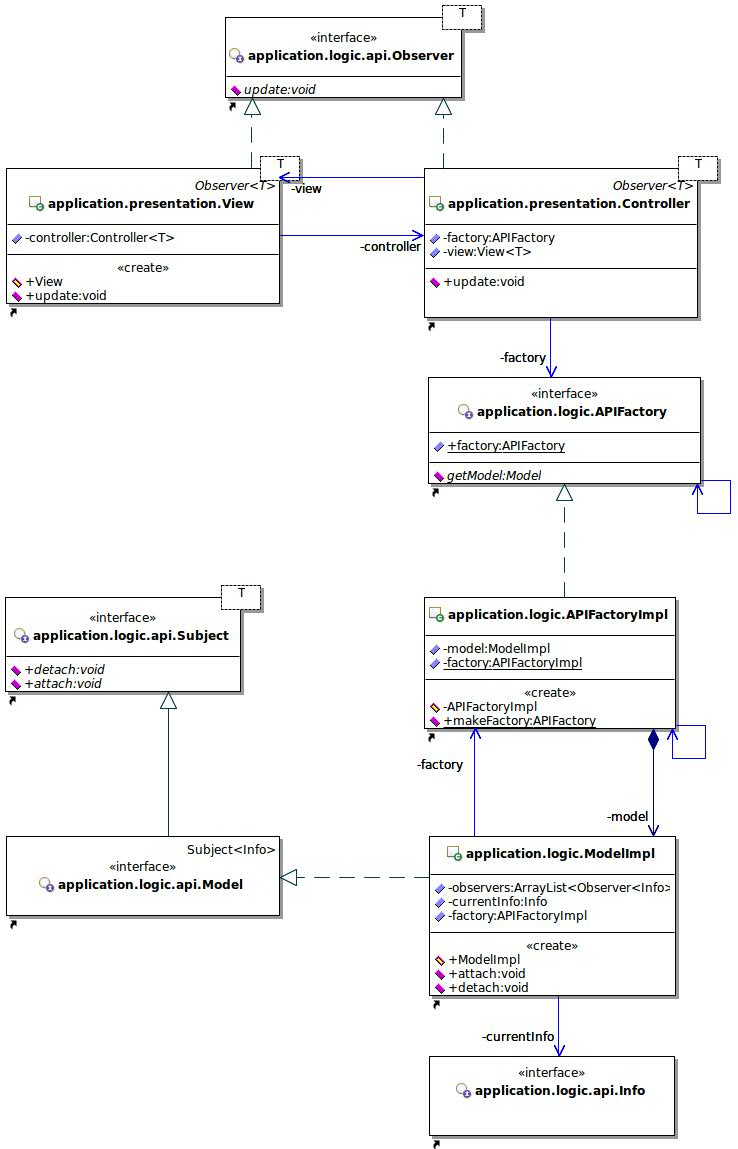
\includegraphics[width=0.6\textwidth]{diagrams/Architecture}
    \caption{Grobe Architektur des Systems}
  \end{center}
\end{figure}

\section{Aufbereitung der Analyse und Systemoperationen}

\subsection{Mockup}

\subsection{System-Use-Case: Spielzug durchführen}
\begin{labeling}[:]{Vorbedingungen}
\item [Akteure] Model, View, Controller
\item [Priorität] Hoch
\item [Beschreibung] Nach dem das Spiel als Anwendung gestartet wurde, wird das Spiel zunächst vorbereitet. Den Spielern wird auf der Konsole mitgeteilt, welcher Spieler aktuell an der Reihe ist und wo sich seine Wissensstreiter befinden. Danach wird der aktuelle Spieler zum Würfeln aufgefordert. Er kann das Würfeln durch einen beliebigen Tastendruck auslösen, wobei dann ein Würfelergebnis zufällig bestimmt wird. Das Würfelergebnis wird ebenfalls auf der Konsole ausgegeben.
Ist das Würfelergebnis gleich 6 und hat der aktuelle Spieler noch einen Wissensstreiter auf dem Heimatfeld und  ist sein Startfeld frei, dann wird ein Wissensstreiter des Spielers auf sein Heimatfeld gestellt. Der Spieler wird darüber auf der Konsole informiert. Ist das Heimatfeld belegt startet eine Fragerunde.
Hat der Spieler alle Wissensstreiter auf dem Pfad, oder er hat eine Augenzahl kleiner als 6 gewürfelt, dann wird ihm eine Auswahlliste seiner Wissensstreiter auf der Konsole präsentiert und er kann durch Eingeben einer Nummer einen Wissensstreiter auswählen, den er versetzen möchte. Sollte der Wissensstreiter auf ein Feld kommen, welches bereits durch einen anderen Wissensstreiter belegt ist, beginnt eine Fragerunde.
Hat der Spieler eine Augenzahl gewürfelt, die kleiner als 6 ist, und hat er noch alle Wissensstreiter auf seinen Heimatfeldern, dann wird er erneut zum würfeln aufgefordert bis er 3 mal in diesem Zug gewürfelt hat.
Alle Eingaben des Spielers werden validiert. Ist eine Eingabe Fehlerhaft wird der Spieler erneut zur Eingabe aufgefordert.
Ein Spieler wird über das Ende seines Zuges auf der Konsole informiert.
\item [Vorbedingungen] Anwendung gestartet, Spiel vorbereitet
\item [Offene Punkte]
\end{labeling}

\subsubsection{Use-Case Diagramm}

\subsubsection{Activity Diagramme}
\begin{figure}[h]
  \begin{center}
    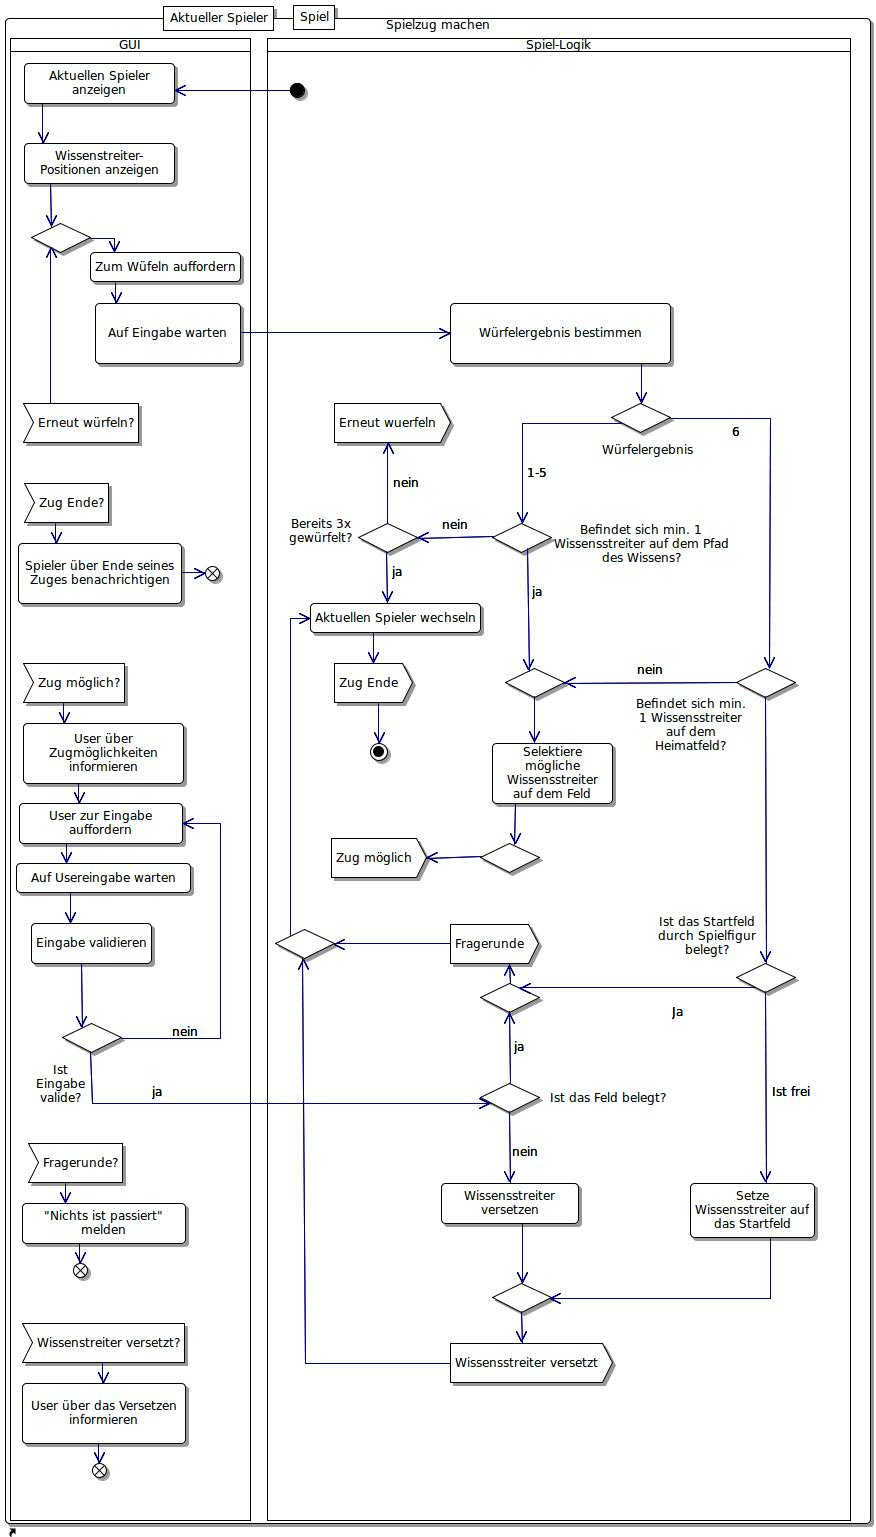
\includegraphics[width=0.8\textwidth]{diagrams/Ablauf_Spielzug_machen_10062016}
    \caption{Aktivity Diagramm für Use-Case \"Spielzug machen\"}
  \end{center}
\end{figure}

\subsection{Schnittstelle der Applikationsschicht}

\subsubsection{System-Sequenz Diagramm}

\subsubsection{Operation: würfeln()}
\begin{labeling}[:]{Verantwortlichkeit}
\item [Parameter] -
\item [Verantwortlichkeit] Es wird eine zufälliges Würfelergebnis bestimmt. 

Ist das Würfelergebnis kleiner als 6 und befindet sich mindestens 1 Wissensstreiter des aktuellen Spielers schon auf dem Pfad, dann wird eine Liste mit allen Wissensstreitern des Spielers, die sich auf dem Pfad befinden, angezeigt. Der Spieler hat dann die Möglichkeit einen Wissensstreiter auszuwählen, indem er die Nummer des Wissensstreiters angibt.

Ist die Augenzahl kleiner als 6, hat der aktuelle Spieler noch nicht 3 mal gewürfelt und es befinden sich noch alle Wissensstreiter des Spielers auf den Heimatfeldern, dann wird der Spieler noch einmal zum Würfeln aufgefordert.

Ist das Würfelergebnis gleich 6 und es befinden sich noch 1 Wissensstreiter des Spielers auf den Heimatfeldern, dann wird, sofern das Startfeld frei ist, ein Wissensstreiter auf das Startfeld gesetzt. Ist das Startfeld belegt, beginnt eine Fragerunde. Danach wird der nächste Spieler ausgewählt und der aktuelle Zug beendet, was durch eine Textausgabe angezeigt wird.

Befinden sich alle Wissensstreiter auf dem Pfad, dann wird ganz unabhängig von der Augenzahl eine Liste mit allen Wissensstreitern, die vom Spieler versetzt werden können, ausgegeben.
Der Spieler hat dann die Möglichkeit einen Wissensstreiter auszuwählen und zu versetzen.
\item [Ausnahmen]
\item [Vorbedingungen] Es gibt einen aktuellen Spieler und der Spieler hat noch nicht 3 mal gewürfelt.
\item [Nachbedingungen] Der Spieler kann einen Wissensstreiter versetzen, oder erneut würfeln, oder es wurde ein Wissensstreiter des Spielers von den Heimatfeldern auf sein Startfeld gezogen bzw. deswegen eine Fragerunde gestartet. Sein Zug ist bei dem letzten Fall dann beendet, sowie der nächste Spieler ist ausgewählt.
\end{labeling}

\subsubsection{Operation: versetzeWissensstreiter(Wissensstreiter)}
\begin{labeling}[:]{Verantwortlichkeit}
\item [Parameter] Ausgewählter Wissensstreiter
\item [Verantwortlichkeit] Ist das Feld auf das der Wissensstreiter gezogen werden soll frei, dann wird er auf dieses Feld gezogen. Ist das Feld belegt beginnt eine Fragerunde.

Nach dem Versetzen oder der Fragerunde wird der Spieler gewechselt und der aktuelle Zug beendet. Das Ende des Zuges wird dem mit einer Nachricht die ausgegeben wird signalisiert.

\item [Ausnahmen]
\item [Vorbedingungen] Der aktuelle Spieler hat einen Wissensstreiter ausgewählt und die Eingabe ist valide. Es existiert eine vom Spieler zuvor gewürfelte Augenzahl.
\item [Nachbedingungen] Der Wissensstreiter wurde versetzt oder eine Fragerunde begonnen. Der nächste Spieler wurde ausgewählt und der Zug des aktuellen Spielers beendet.
\end{labeling}

\section{Zustandsautomaten}

\section{Detailed Design und das Objektmodell}

\subsection{Sequenz- und Kommunikationsdiagramm}

\subsection{Design-Objektmodeel}

\section{Implementierung der Oberfläche}


\end{document}
